
\documentclass[graybox, envcountchap, twocolumn]{styles/svmult}
\usepackage{fontspec}  % For custom fonts
\usepackage{polyglossia}  % For language support

% Set English and Bangla as languages
\setdefaultlanguage{english}
\setotherlanguage{bengali}

% Set fonts for English and Bangla
\newfontfamily\bengalifont[Script=Bengali]{Kalpurush}  % You can change 'Kalpurush' to another Bangla font like 'SolaimanLipi' or 'Noto Sans Bengali'

\usepackage{amssymb,amsmath,bm}
\DeclareMathAlphabet{\mathcal}{OMS}{cmsy}{m}{n}
\usepackage{textcomp}
\newcommand\abs[1]{\left\lvert#1\right\rvert}
\usepackage{longtable}
\usepackage{algorithm2e}
\usepackage{tocbibind}
\usepackage[toc]{multitoc}
\renewcommand{\bibname}{References}
\usepackage{mathptmx}  % Times Roman as basic font
\usepackage{helvet}    % Helvetica as sans-serif font
\usepackage{courier}   % Courier as typewriter font

\usepackage{makeidx}   % Index generation
\usepackage{graphicx}  % Standard LaTeX graphics tool
\usepackage[justification=centering]{caption}
\usepackage{subfig}
\usepackage{multicol}  % For multi-column index
\usepackage{multirow}
\usepackage[bottom]{footmisc}  % Footnotes at the bottom
\usepackage[bookmarksnumbered=true,
            bookmarksopen=true,
            colorlinks=true,
            linkcolor=blue,
            anchorcolor=blue,
            citecolor=blue]{hyperref}

\graphicspath{{figures/}}

\makeindex  % For subject index generation

\begin{document}

\title{Probability}
{\bengalifont
\section{Frequentists vs. Bayesians}
প্রবাবিলিটি বা সম্ভাব্যতা কাকে বলে?
% what is probability? 

একদিকে প্রবাবিলিটিকে  \textbf{ফ্রিকোয়েন্টিস্ট} এর আলোকে ব্যাখ্যা করা হয়; যেখানে সম্ভাব্যতা (probability) কোনো ঘটনার দীর্ঘমেয়াদি পুনরাবৃত্তির হারকে বোঝায়। উদাহরণস্বরূপ, আমরা যদি একটা কয়েনকে অনেকবার ছুঁড়ি, তবে ধারণা করা হয় এটি প্রায় অর্ধেক সময় "হেডস" পড়বে।

প্রবাবিলিটির আরেকটা ব্যাখ্যা দাড় করানো হয় \textbf{বায়েসিয়ান}(Bayesian) ব্যাখ্যার ভিত্তিতে। এই ব্যাখ্যায়, সম্ভাব্যতা আমাদের কোনো ঘটনার প্রতি \textbf{অনিশ্চয়তা} বোঝাতে ব্যবহৃত হয়; অর্থাৎ, এটি পুনরাবৃত্তি করা পরীক্ষার উপর নির্ভর না করে ডাটা বা ইনফর্মেশনের সঙ্গে সম্পর্কিত। বায়েসিয়ান সংজ্ঞার ভিত্তিতে কয়েন পরবর্তী বার ছুড়ে মারলে "হেডস" বা "টেলস" পড়ার সমান সম্ভাবনা রয়েছে।    


বায়েসিয়ান ব্যাখ্যার একটা বড় সুবিধা হল, এটি এমন সব ঘটনার অনিশ্চয়তা(uncertainty) মডেল করতে পারে যেগুলোর পুনরাবৃত্তি নাও হতে পারে।  উদাহরণস্বরূপ, আমরা ২০২০ সালের মধ্যে মেরু বরফ গলে যাবে কিনা তা নিয়ে সম্ভাব্যতা নির্ণয় করতে চাই; এই ঘটনা ঘটলে সর্বোচ্চ একবার হতে পারে বা একদম নাও হতে পারে; কিন্তু বারবার হবে না। কিন্তু তবুও এরকম শূন্য/একবার ঘটে যাওয়া ঘটনার অনিশ্চয়তা নির্ণয় করতে হতে পারে। 
মেশিন লার্নিং ভিত্তিক আরেকটা ঘটনার আলোকে ব্যাপারটা ব্যাখ্যা করা যাক। ধরি,  আমরা রাডারে একটি "ব্লিপ" দেখেছি এবং এর ভিত্তিতে আমরা লক্ষ্যবস্তুর অবস্থান (যা হয়তো একটি পাখি, বিমান বা ক্ষেপণাস্ত্র হতে পারে) সম্পর্কে probability distribution নির্ণয় করতে চাই। এই ক্ষেত্রে, পুনরাবৃত্তি করা পরীক্ষার ধারণা প্রাসঙ্গিক নয়, কিন্তু বায়েসিয়ান ব্যাখ্যা স্বাভাবিক এবং যথাযথ।

এই বইয়ে আমরা বায়েসিয়ান ব্যাখ্যার ভিত্তিতেই সব আলোচনা করব। }




\section{Probability theory- {\bengalifont এর একটি সংক্ষিপ্ত পর্যালোচনা}}

{\bengalifont ধরি $𝑋$ কোনো অজানা পরিমাণকে নির্দেশ করছে, যেমন একটা লুডুর ডাইস গড়ালে সেটা কোন দিক পড়বে তা বের করতে হবে। এরকম একটা random ঘটনার সম্ভাব্য ফলাফল বোঝাতে $X$ চিহ্নের ব্যবহার করা হয়; যেখানে $X$ ডিসক্রিট(Discrete) বা কন্টিনিউয়াস(Continuous) হতে পারে।  }

\subsection{{\bengalifont ব্যাসিক কনসেপ্ট}}

{\bengalifont
\textbf{Discrete random variable}: $X$ একটা সীমিত(finite) গণনাযোগ্য অসীম সেট(countably infinite set) থেকে মান গ্রহণ করে। যেমন কয়েন ছুড়ে টস করার পর কতবার হেডস এসেছে সেটা ডিসক্রিট নাম্বার (10,13,78,..)


\textbf{Continuous random variable}:  $X$ এর মান একটি নির্দিষ্ট সীমার মধ্যে যেকোনো বাস্তব সংখ্যা (Real numbers) হবে। যেমন একটা স্থানের মানুষদের উচ্চতা কন্টিনিউয়াস (5.3 ft, 6.0 ft )}

\textbf{Probability Distribution}: {\bengalifont একটা random variable-এর সম্ভাব্য সকল মান পড়ার সম্ভাবনাকে একত্র করলে,সেটাকে প্রবাবিলিটি ডিস্ট্রিবিউশন বলছে। discrete value এর জন্যে একে PMF বলে এবং continious value এর ক্ষেত্রে PDF বলে, যেটা আমরা পরের সেকশনে বিস্তারিত জানতে পারবো ।

লুডুর ডাইসের কথা চিন্তা করা যাক, যেখানে একবার ৬ পড়ার সম্ভাবনা $P(X)$= ১/৬; সকল মানকে একসাথে যদি আমরা একটা গ্রাফে বসায় যেখানে $x$-অক্ষ বরর্বর ডাটা পয়েন্ট থাকবে, আর তাদের এককভাবে আসার সম্ভাবনা $Y$-অক্ষ বরাবর রেখে মান বসালে যেই সম্পূর্ণ স্পেইসটা পাবো সেটাই probabilty distribution }

\subsubsection{CDF: cumulative distribution function}
{\bengalifont একটা random variable} $X$ {\bengalifont এর ভিন্ন মান পাওয়ার প্রবাবিলিটি ডিস্ট্রিবিউশন কেমন হবে সেটা জানার জন্যে CDF ব্যবহার করা যায় যাকে} $𝐹(𝑥)$ {\bengalifont এর মাধ্যমে প্রকাশ করা হয়। }

\begin{equation}
F(x) \triangleq P(X \leq x)=\begin{cases}
\sum_{u \leq x}p(u) & \text{, discrete}\\
\int_{-\infty}^{x} f(u)\mathrm{d}u & \text{, continuous}\\
\end{cases}
\end{equation}


- $  P(X \leq x) $ $X$ -{\bengalifont এর মান} $x$-{\bengalifontএর কম বা সমান হওয়ার সম্ভাবনা।}

- $p(u)$ {\bengalifont হচ্ছে ডিসক্রিট ভ্যারিয়েবেলের জন্যে  প্রবাবিলিটি মাস ফাংশন (Probability Mass Function, PMF), যা $u$ এর একটি নির্দিষ্ট মান পাওয়ার সম্ভাব্যতা প্রকাশ করে }

- $ f(u)$ {\bengalifont হচ্ছে কন্টিনিউয়াস ভ্যারিয়েবেলের জন্যে প্রবাবিলিটি ডেনসিটি ফাংশন (probability density function), $u$ এর সম্ভাব্যতা। } 



\subsubsection{PMF {\bengalifont এবং} PDF}
\paragraph{PMF: Probability Mass Function}
{\bengalifont
Random Variable $X$ এর নির্দিষ্ট মান পাওয়ার সম্ভাবনা কতটুকু, সেটা নির্ধারন করা হয় Probability Mass Function (PMF) এর মাধ্যমে। উদাহরণস্বরূপ,  যদি একটি ৬-পাশের ডাইস ফেলা হয় , প্রবাবিলিটি মাস ফাংশন (Probability Mass Function, PMF) প্রতিটি পাশের সম্ভাবনা নির্দেশ করবে, যার মান ১ থেকে ৬ এর মধ্যে আসবে।
}
\begin{itemize}
    \item PMF,  $p(x)$ = $P(X=x)$ {\bengalifont হিসাবে প্রকাশ করা হয়, যা নির্দেশ করে random ভেরিয়েবল} $X$ {\bengalifont একটি নির্দিষ্ট মান } $x$ {\bengalifont নেওয়ার সম্ভাবনা। }
    \item {\bengalifont বৈশিষ্ট্য:}
    \begin{itemize}
        \item $0 ≤ p(x) ≤ 1$ {\bengalifont (সম্ভাবনা ০ এবং ১-এর মধ্যে থাকে)}
        \item $\sum_{x \in X} p(x) = 1$ {\bengalifont (সব সম্ভাবনার যোগফল ১ হয়)}
    \end{itemize}
\end{itemize}


\paragraph{PDF: Probability Density Function}
% \subsubsection[short]{PDF: Probability Density Function}

{\bengalifont Probability Density Function (PDF) continuous random variable-এর probability density নির্দেশ করে। এটা ব্যবহার করা হয় একটি নির্দিষ্ট সীমার মধ্যে সম্ভাবনা বের করার জন্য। }
% যেহেতু ভেরিয়েবলটি অসীম মান গ্রহণ করতে পারে, নির্দিষ্ট একটি মান নেওয়ার সম্ভাবনা শূন্য হয়।}

\begin{itemize}
    \item $P(a \leq X \leq b) = \int_{a}^{b} f(x) \, dx$ {\bengalifont (এখানে $f(x)$ হল PDF, যা probability density নির্দেশ করে)}
    \item {\bengalifont বৈশিষ্ট্য:}
    \begin{itemize}
        \item $f(x) \geq 0$ {\bengalifont (density  শূন্য বা তার বেশি হয়)}
        \item $\int_{-\infty}^{\infty} f(x) \, dx = 1$ {\bengalifont ( পুরো density value ১ হয়)}
    \end{itemize}
\end{itemize}


% {\bengalifont এটি $X$-এর সম্ভাবনা ঘনত্ব নির্দেশ করে, যেখানে $X$ এর গড় ০ এবং মানদণ্ড ১।}
% For discrete random variable, We denote the probability of the event that $X=x$ by $P(X=x)$, or just $p(x)$ for short. Here $p(x)$ is called a \textbf{probability mass function} or \textbf{PMF}.A probability mass function is a function that gives the probability that a discrete random variable is exactly equal to some value\footnote{\url{http://en.wikipedia.org/wiki/Probability_mass_function}}. This satisfies the properties $0 \leq p(x) \leq 1$ and $\sum_{x \in \mathcal{X}} p(x)=1$.

% For continuous variable, in the equation $F(x)=\int_{-\infty}^{x} f(u)\mathrm{d}u$, the function $f(x)$ is called a \textbf{probability density function} or \textbf{PDF}. A probability density function is a function that describes the relative likelihood for this random variable to take on a given value\footnote{\url{http://en.wikipedia.org/wiki/Probability_density_function}}.This satisfies the properties $f(x) \geq 0$ and $\int_{-\infty}^{\infty} f(x)\mathrm{d}x=1$.

\subsection{Multivariate random variables}
% \textbf{Joint Distribution: }
% {\bengalifont দুইটি random variable-এর একসাথে ঘটার সম্ভাবনাকে জয়েন্ট প্রবাবিলিটি বলে, যেমন একটা ডাইসের ২ পড়ার এবং কয়েনের হেডস পড়ার সম্ভাবনা। }

\textbf{Marginal Distribution}
{\bengalifont অন্য ভ্যারিয়েবলের মান বিবেচনা না করে, একটা random ভ্যারিবেলের নির্দিষ্ট মান আসার সম্ভাবনা,যেমন ডাইসে ২ আসার সম্ভাবনা, কয়েন টসের ফল কি হবে সেটা বিবেচনা না করে।
ডিসক্রিট এর ক্ষেত্রে - }
\begin{equation}
    P(X = x) = \sum_y P(X = x, Y = y)
\end{equation} 
{\bengalifont কন্টিনিউয়াস এর ক্ষেত্রে }- 
\begin{equation}
    P(X = x) = \int_{-\infty}^{+\infty} f(x, y) \, dy
\end{equation}

\subsubsection{Joint CDF}
{\bengalifont দুটি random variable $X$ এবং $Y$ এর জন্যে } CDF- 
\[
F(x,y) \triangleq P(X \leq x \cap Y \leq y)=P(X \leq x , Y \leq y)
\]
\begin{equation}
F(x,y) \triangleq P(X \leq x, Y \leq y) = \begin{cases}
\sum_{u \leq x, v \leq y} p(u,v) & \text{(discrete)} \\
\int_{-\infty}^{x} \int_{-\infty}^{y} f(u,v)\mathrm{d}u \mathrm{d}v & \text{(continuous)}
\end{cases}
\end{equation}

-  $F(x, y)$ { \bengalifont হচ্ছে joint CDF, {\bengalifont যেখানে  $X$ এবং $Y$ এর মান $x$ এবং $y$ এর কম বা সমান হওয়ার সম্ভাবনা কত নির্ধারন করে ।}}

-  $\sum_{u \leq x, v \leq y} p(u, v)$ {\bengalifont হচ্ছে ডিসক্রিট দুইটি random variable-এর PMF}

-  $\int_{-\infty}^{x} \int_{-\infty}^{y} f(u, v) \, du \, dv$ {\bengalifont হচ্ছে কন্টিনিউয়াস ভ্যারিয়েবেলের ক্ষেত্রে pdf ইন্টিগ্রেশন।}


\subsubsection{Product Rule}

 {\bengalifont দুটি ঘটনা একসাথে ঘটার সম্ভাবনাকে প্রকাশ করা যায় Product Rule এর মাধ্যমে।  প্রোডাক্ট রুলকে conditional probability ($P(X,Y)$) এবং marginal probability ($P(Y)$) এর গুণফলের মাধ্যমে প্রকাশ করা হয়।   }
\begin{equation}\label{eqn:product-rule}
p(X,Y) = P(X|Y) P(Y)
\end{equation} 


-   $P(X \cap Y)$ {\bengalifont বোঝায়} $X$ {\bengalifont এবং} 

-   $P(X \mid Y)$ {\bengalifont বোঝায়} $Y$ {\bengalifontঘটে যাওয়ার শর্তে,} $X$ {\bengalifont ঘটার সম্ভাবনা} 

-   $P(Y)$ {\bengalifont হলো} $Y$ {\bengalifont ঘটার সম্ভাবনা।} \end{itemize}


\subsubsection{Chain Rule}
{\bengalifont চেইন রুল প্রোডাক্ট রুল এর একটি সম্প্রসারণ যা একাধিক ঘটনার সম্ভাবনাকে একত্রে প্রকাশ করে। কমপ্লেক্স প্রবাবিলিটি বা মেশিন লার্নিং (backpropagation concept) এর ক্ষেত্রে চেইন রুল ব্যবহার করা হয়। }
\begin{equation}
p(X_{1:N}) = p(X_1)p(X_2|X_1)p(X_3|X_2,X_1)...p(X_N|X_{1:N-1})
\label{eq:1}
\end{equation}



-   {\bengalifont এখানে 
    n সংখ্যক ঘটনার একসাথে ঘটার সম্ভাবনা নির্ণয় করতে আমরা প্রতিটি ঘটনার কন্ডিশনাল প্রবাবিলিটি গুণ করছি }



\subsubsection{Marginal Distribution} {\bengalifont Marginal Distribution variable এর সেট থেকে কেবলমাত্র একটা ভ্যারিয়েবলকে ফোকাসে রেখে তার probability distirbution নির্ণয় করে অন্য সকল ভ্যারিয়েবল বাদ রেখে।  যেমন, random variable $X$ এর marginal CDF নির্ণয় করার সময় $X$ এর মান শুধুই $x$ এর সমান বা কম বিবেচনা করা হবে, $Y$ এর মান যাই থাকুক না কেন।  }

$X$ {\bengalifont এর জন্যে } \textbf{Marginal CDF}:

{\bengalifont Discrete case এবং continuous case এর জন্যে marginal CDF-  }

\begin{equation}\begin{split}
F_X(x) \triangleq F(x,+\infty) = 
\begin{cases}
\sum\limits_{x_i \leq x} P(X=x_i) = \sum\limits_{x_i \leq x} \sum\limits_{j=1}^{+\infty} P(X=x_i,Y=y_j) \\
\int_{-\infty}^{x} f_X(u)du = \int_{-\infty}^{x} \int_{-\finite}^{+\infty} f(u, v) du dv
\end{cases}
\end{split}\end{equation}


    - {\bengalifont প্রথম ক্ষেত্রে, যখন random variable discrete হয়, তখন আমরা $X$ এর সকল  $x_i$ মানের জন্য $P(X=x_i)$ সম্ভাবনা নির্ণয় করে summation বের করছি, যেখানে $x_i <_ x $ ; দ্বিতীয় summation এর ক্ষেত্রে, $Y$ এর সকল মানের জন্যে পাওয়া joint probability $P(X=x_i,Y=y_j)$ sum up করছে।   }

    - {\bengalifont দ্বিতীয় ক্ষেত্রে, যখন random variable continuous হয়, তখন আমরা joint probability density function $f(u,v)$ কে ইন্টিগ্রেট করছি প্রথমে $v$ এর সাপেক্ষে (অর্থাৎ $Y$ এর সম্ভাব্য সকল মান নিয়ে), অতপর $u$ এর সাপেক্ষে।}

$Y$ {\bengalifont এর জন্যে } \textbf{Marginal CDF}:

\begin{equation}\begin{split}
F_Y(y) \triangleq F(+\infty, y) = 
\begin{cases}
\sum\limits_{y_j \leq y} P(Y=y_j) = \sum\limits_{i=1}^{+\infty} \sum\limits_{y_j \leq y} P(X=x_i,Y=y_j) \\
\int_{-\infty}^{y} f_Y(v) dv = \int_{-\infty}^{+\infty} \int_{-\infty}^{y} f(u, v) du dv
\end{cases}
\end{split}\end{equation}

-   {\bengalifont প্রথম ক্ষেত্রে, আমরা $Y$ এর মান $y_j \leq y$ এর জন্য $P(Y=y_j)$ এর সম্ভাবনা বের করি। এই সম্ভাবনাটি $X=x_i$ এবং $Y=y_j$ এর joint probability নির্ণয় করে, এবং এটি সব $y_j \leq y$ এর প্রবাবিলিটি sum  up করে। }

-   {\bengalifont দ্বিতীয় ক্ষেত্রে, যখন $Y$ একটি continuous random ভেরিয়েবল হয়, তখন আমরা joint  probability definitions function  $f(u, v)$ ইন্টিগ্রেট করে $Y \leq y$ এর সম্ভাবনা বের করি। এটি সমস্ত $X$ এর জন্য এবং $Y$ এর নির্দিষ্ট মান পর্যন্ত সম্ভাবনাকে ইন্টিগ্রেট করে।}



\textbf{Marginal PMF & PDF}:

\begin{equation} \begin{cases}
P(X=x_i)=\sum_{j=1}^{+\infty}P(X=x_i,Y=y_j) & \text{, discrete}\\
f_X(x)=\int_{-\infty}^{+\infty} f(x,y)\mathrm{d}y & \text{, continuous}\\
\end{cases}\end{equation}

\begin{equation}\begin{cases}
p(Y=y_j)=\sum_{i=1}^{+\infty}P(X=x_i,Y=y_j) & \text{, discrete}\\
f_Y(y)=\int_{-\infty}^{+\infty} f(x,y)\mathrm{d}x & \text{, continuous}\\
\end{cases}\end{equation}


\subsubsection{Conditional distribution}
{\bengalifont একটা ঘটনার প্রভাবে আরেকটি ঘটনা ঘটার সম্ভাব্যতাকে conditional distribution দ্বারা প্রকাশ করা হয়। যদি $ Y = y_j$ হয়, তবে $X = x_i$ হওয়ার সম্ভাবনাকে প্রকাশ করা যায় -}
\textbf{Conditional PMF}:
\begin{equation}
p(X=x_i|Y=y_j)=\dfrac{p(X=x_i,Y=y_j)}{p(Y=y_j)} \text{ if } p(Y)>0
\end{equation}

-   $\dfrac{p(X=x_i,Y=y_j)}{p(Y=y_j)}, X & Y $ {\bengalifont এর জয়েন্ট প্রবাবিলিটি }

-   $p(Y=y_j), Y $ {\bengalifont এর মার্জিনাল প্রবাবিলিটি  }
\end{itemize}
pmf $p(X|Y)$ {\bengalifont কে বলা হয়} \textbf{conditional probability}.

\textbf{Conditional PDF}:
\begin{equation}
f_{X|Y}(x|y)=\dfrac{f(x,y)}{f_Y(y)}
\end{equation}

-   $ p(X=x_i,Y=y_j), X & Y $ {\bengalifont এর } joint probability

-   $p(Y=y_j), Y $ {\bengalifont এর মার্জিনাল প্রবাবিলিটি  }



\subsection{Bayes rule}
{\bengalifont কন্ডিশনাল প্রবাবিলিটির মধ্যে সম্পর্ক প্রকাশ করার জন্যে Bayes Rule ব্যবহার করা হয় যেখানে নতুন ইনফর্মেশনের ভিত্তিতে একটা ঘটনার প্রববিলিটিকে আপডেট করা হবে। মেশিন লার্নিং এ, বিশেষত প্রোবাবিলিস্টিক মডেল যেমন Naive Bayes ক্লাসিফায়ার এই নিয়ম ব্যবহার করা হয়। }
\begin{equation}
\begin{split}
p(Y=y|X=x) & =\dfrac{p(X=x,Y=y)}{p(X=x)} \\
           & =\dfrac{p(X=x|Y=y)p(Y=y)}{\sum_{y'}p(X=x|Y=y')p(Y=y')}
\end{split}
\end{equation}

-   {\bengalifont 
    \(p(X=x, Y=y)\) হল \(Y=y\) হওয়ার সম্ভাবনা, যখন \(X=x\) হবে ; এখানে \(p(X=x, Y=y)\)  কন্ডিশনাল প্রবাবিলিটি  এবং \(p(X=x)\) হল মার্জিনাল প্রবাবিলিটি ।  
    }

-    {\bengalifont 
    দ্বিতীয় সমীকরণে, আমরা প্রোডাক্ট রুল ব্যবহার করেছি, যেখানে \(p(X=x|Y=y)\) যখন  \(Y=y\) হবে তখন \(X=x\) হওয়ার সম্ভাবনা এবং \(p(Y=y)\) হলো $X$ এর কোন ইনফরমেশন ছাড়া  মার্জিনাল প্রবাবিলিটি ।
    }

-   {\bengalifont 
    denominator -এ থাকা \(\sum_{y'} p(X=x|Y=y') p(Y=y')\) হলো নরমালাইজেশন ফ্যাক্টর যেখানে $X = x$ এর জন্য  \(Y\)-এর সম্ভাব্য মান নিয়ে summation করা হয় । 
    }


%%%%%%%%%%%%%%%%%%%%%%%%%%%%%%%%%%%%%%%%%%%%%%%%%%%%%%%%%%%%%%%%%%%%%%%%%%%%%%%%%%%%%%%%%%%

\subsection{Independence \& conditional independence}
{\bengalifont 
\(X\) এবং \(Y\) unconditional বা marginally independent হবে, যদি তাদের joint probability কে তাদের marginal probability-র গুণফল এর মাধ্যমে প্রকাশ করা যায়। Unconditional independence \(X \perp Y\) সিম্বলের মাধ্যমে প্রকাশ করা হয়; যেখানে - }
\begin{equation}
X \perp Y = P(X,Y) = P(X)P(Y)
\end{equation}

-   {\bengalifont সমীকরণে , \(X\) এবং \(Y\) একে অপরের উপর নির্ভরশীল নয়, তাদের মধ্যে কোনো সরাসরি  সম্পর্ক নেই। একসাথে \(X\) এবং \(Y\)-এর joint probability, তাদের marginal probability \(P(X)\) এবং \(P(Y)\)-এর গুণফল দিয়ে প্রকাশ করা সম্ভব। }

-   {\bengalifont 
অন্যদিকে , \(X\) এবং \(Y\) conditionally independent (CI) হবে, যদি আরও একটি variable \(Z\) এর উপস্থিতি থাকে । এটি প্রকাশ করা হয়:}
% মানে, \(Z\) জানার পর \(X\) এবং \(Y\) একে অপরের উপর নির্ভরশীল নয়। 
\begin{equation}
X \perp Y|Z = P(X,Y|Z) = P(X|Z)P(Y|Z)
\end{equation}

-   {\bengalifont এখানে যদি \(Z\) ঘটার সম্ভাবনা থাকে, তবে  \(X\) এবং \(Y\) এর মধ্যে কোনো সম্পর্ক থাকে না । \(Z\) এর সাথে তাদের conditional probability থাকার শর্তে, নিজেদের মধ্যে joint probability থাকছে;  পরের ইকুয়েশনে এই শর্তে তাদের marginal probabilities দিয়ে প্রকাশ করা যায়। }


\subsection{Quantiles}
\bengalifont 
যেহেতু cdf \(F\) একই প্যাটার্নে (monotonic) বাড়তে থাকা ফাংশন, এর একটি inverse আছে, যা \(F^{-1}\) মাধ্যমে প্রকাশ করা যায়। যদি \(X\)-এর cdf \(F\) হয় , তাহলে \(F^{-1}(\alpha)\) হল \(x_{\alpha}\)-এর সেই মান যেখানে \(P(X \leq x_{\alpha}) = \alpha\)। একে বলা হয় \(F\)-এর \(\alpha\) quantile। \(F^{-1}(0.5)\)-এর মানকে বলা হয় distribution-এর \textbf{median}, যেখানে বামপাশে এবং ডানপাশে probability সমানভাবে ভাগ করা থাকে। \(F^{-1}(0.25)\) এবং \(F^{-1}(0.75)\) lower এবং upper \textbf{quartiles}।

\subsection{Mean & variance}
\bengalifont 
একটি distribution-এর সবচেয়ে পরিচিত বৈশিষ্ট্য হল তার \textbf{mean} (গড়) বা \textbf{expected value}, যা \(\mu\) দিয়ে প্রকাশ করা হয়। discrete random variable-এর জন্য mean কে সংজ্ঞায়িত করা হয়:
\[
\mathbb{E}[X] \triangleq \sum_{x \in \mathcal{X}}x p(x)
\]

 \textbf{\(\mathbb{E}[X]\)} {\bengalifont দ্বারা \(X\) এর expected value বা গড় প্রকাশ করা হয়}

এবং continuous variable-এর জন্য:
\[
\mathbb{E}[X] \triangleq \int_{\mathcal{X}}x p(x) \mathrm{d}x
\]
যদি এই ইন্টিগ্রাল finite না হয়, তাহলে mean নির্ধারণ করা যায় না।

\bengalifont 
\textbf{Variance} হল একটি distribution-এর "spread" বা বিচরণ পরিমাপ। এটি \(\sigma^2\) দিয়ে প্রকাশ করা কতখানি দূরে আছে তা পরিমাপ করে ।  variance এর সংজ্ঞা দেয়া হয়:
\begin{align}
var[X]& =\mathbb{E}[(X-\mu)^2] \\
      & =\int{(x-\mu)^2p(x)\mathrm{d}x} \nonumber \\
      & =\int{x^2p(x)\mathrm{d}x}+{\mu}^2\int{p(x)\mathrm{d}x}-2\mu\int{xp(x)\mathrm{d}x} \nonumber \\
	  & =\mathbb{E}[X^2]-{\mu}^2
\end{align}



-   {\bengalifont প্রথম অংশে \(\mathbb{E}[(X-\mu)^2]\) মানে, আমরা \(X\) এর মান থেকে এর গড় \( \mu \) বাদ দিয়ে তার স্কোয়ারের গড় নিচ্ছি।}


-   {\bengalifont এরপর এইটাকে আমরা \(\int (x-\mu)^2 p(x) \, \mathrm{d}x\) এর মাধ্যমে প্রকাশ করি, যেখানে \(p(x)\) হলো \(X\) এর probability density function।}



-   {\bengalifont তৃতীয় ক্ষেত্রে,  \(\int x^2 p(x) \, \mathrm{d}x\) হলো \(X\) এর স্কোয়ার করা মানগুলোর expected value।}


-   {\bengalifont \(\mu^2 \int p(x) \, \mathrm{d}x\) অংশটি গড়ের স্কোয়ারের গড় প্রকাশ করছে, আর \(2\mu \int x p(x) \, \mathrm{d}x\) হলো গড় ও \(X\) এর মানের সম্পর্ক।}


-   {\bengalifont সবশেষে, আমরা দেখতে পাই \(\mathbb{E}[X^2] - \mu^2\), যা হলো variance এর সংক্ষিপ্ত ফর্ম }

\bengalifont 
এখান থেকে আমরা একটি গুরুত্বপূর্ণ ফলাফল পাই:
\begin{equation}
\mathbb{E}[X^2]=\sigma^2+{\mu}^2
\end{equation}

\bengalifont 
\textbf{Standard deviation} কে সংজ্ঞায়িত করা হয়:
\begin{equation}
std[X] \triangleq \sqrt{var[X]}
\end{equation}
\bengalifont 
এটা কাজে লাগে কারণ এটি \(X\)-এর সাথে একই একক (units) থাকে।

\section{{\bengalifont কিছু সাধারণ ডিসক্রিট ডিস্ট্রিবিউশন}}

{\bengalifont
এই অংশে আমরা কিছু সাধারণত ব্যবহৃত প্যারামেট্রিক ডিস্ট্রিবিউশন আলোচনা করবো, যা ডিসক্রিট স্টেট স্পেসের উপর ভিত্তি করে, কিছু ফাইনাইট এবং কাউন্টেবল ইনফিনিট।}

\subsection{{\bengalifont Barnouli  এবং Binomial Distribution}}

\begin{definition}
\bengalifont
ধরি  আমরা একটি কয়েন একবার ছুঁড়লাম। $X \in \{0,1\}$ হলো একটি binary random variable, যেখানে "হেডস" পাওয়ার সম্ভাবনা $\theta$। তখন আমরা বলি যে $X$ এর \textbf{Barnouli Distribution} আছে। এটা লেখা হয় $X \sim \text{Ber}(\theta)$, যেখানে pmf (Probability Mass Function) এর সংজ্ঞা দেয়া হয় এভাবে:

\begin{equation}
\text{Ber}(x|\theta) \triangleq \theta^{\mathbb{I}(x=1)}(1-\theta)^{\mathbb{I}(x=0)}
\end{equation}
\end{definition}

\bengalifont
- $X$ হলো র‍্যান্ডম ভ্যারিয়েবল, যা ০ অথবা ১ হতে পারে (মানে হেডস বা টেইলস পাওয়া গেল কিনা)।

- $\theta$ হলো হেডস পাওয়া সম্ভাবনা।

- $\mathbb{I}(x=1)$ একটি ইন্ডিকেটর ফাংশন, যা তখন ১ হবে যখন $x=1$, আর বাকি সব ক্ষেত্রে ০।

- $\theta^{\mathbb{I}(x=1)}$ এই টার্মটি তখন কাজ করবে যখন $x = 1$, আর $1 - \theta^{\mathbb{I}(x=0)}$ কাজ করবে যখন $x = 0$।

\begin{definition}
ধরি আমরা $n$ বার কয়েন ছুঁড়লাম। $X \in \{0,1,\cdots,n\}$ হলো হেডসের সংখ্যা। যদি হেডস পাওয়ার সম্ভাবনা $\theta$ হয়, তাহলে $X$ এর \textbf{Binomial Distribution} আছে, যা প্রকাশ করা হয় $X \sim \text{Bin}(n, \theta)$। এর pmf হলো:
\begin{equation}\label{eqn:binomial-pmf}
\text{Bin}(k|n,\theta) \triangleq \dbinom{n}{k}\theta^k(1-\theta)^{n-k}
\end{equation}
\end{definition}

\bengalifont
- $\dbinom{n}{k}$ এই টার্মটি কম্বিনেশন বোঝায়, মানে $n$ বার ট্রায়াল থেকে $k$ বার হেডস পাওয়ার সম্ভাব্য উপায়

- $\theta^k$ বোঝায় $k$ বার হেডস পাওয়ার সম্ভাবনা।

- $(1-\theta)^{n-k}$ হলো বাকি $n-k$ বার টেইলস পাওয়ার সম্ভাবনা।

- পুরো ফর্মুলা বলতে চায় $k$ বার সফলতা পাওয়ার সম্ভাবনা কী, যেখানে $n$ বার কয়েন ছুঁড়া হয়েছে।

\subsection{{\bengalifont multinoulli এবং multinomial distribution}}

\begin{definition}
\bengalifont
Barnouli Distribution একবার কয়েন ছুঁড়া মডেল করে। কিন্তু যদি $K$-পাশওয়ালা একটি লুডুর ডাইস ছুঁড়তে হয়, তখন $\vec{x} =(\mathbb{I}(x=1),\cdots,\mathbb{I}(x=K)) \in \{0,1\}^K$ হবে একটি random vector (এটা \textbf{dummy encoding} বা \textbf{one-hot encoding} নামে পরিচিত), তখন বলা হয় $X$ এর \textbf{multinoulli distribution} (বা \textbf{categorical distribution}) আছে, প্রকাশ করা হয় $X \sim \text{Cat}(\theta)$। pmf হলো:

\begin{equation}
p(\vec{x}) \triangleq \prod\limits_{k=1}^K\theta_k^{\mathbb{I}(x_k=1)}
\end{equation}
\end{definition}

\bengalifont
- এক্ষেত্রে $\vec{x}$ একটি one-hot encoding vector, যেটা দেখায় কোন সাইডে (১ থেকে $K$) ডাইস পড়লো।

- $\theta_k$ হলো $k$-তম সাইডে ডাইস পড়ার সম্ভাবনা।

- $\prod\limits_{k=1}^K\theta_k^{\mathbb{I}(x_k=1)}$ বোঝায় সেই সাইডে (কোন একটা নির্দিষ্ট $k$) ডাইস পড়ার সম্ভাবনা।

\begin{definition}
\bengalifont
ধরি আমরা $K$-পাশওয়ালা ডাইস $n$ বার ছুঁড়লাম। $\vec{x} =(x_1,x_2,\cdots,x_K) \in \{0,1,\cdots,n\}^K$ হলো একটি random vector, যেখানে $x_j$ হলো $j$-তম সাইডে কতবার ডাইস পড়েছে। তখন বলা হয় $X$ এর \textbf{মাল্টিনোমিয়াল ডিস্ট্রিবিউশন} আছে, লেখা হয় $X \sim \text{Mu}(n, \vec{\theta})$। pmf হলো:
\begin{equation}\label{eqn:multinomial-pmf}
p(\vec{x}) \triangleq \dbinom{n}{x_1 \cdots x_k} \prod\limits_{k=1}^K\theta_k^{x_k}
\end{equation}
যেখানে $\dbinom{n}{x_1 \cdots x_k} \triangleq \dfrac{n!}{x_1!x_2! \cdots x_K!}$
\end{definition}

- $\dbinom{n}{x_1 \cdots x_k}$ বোঝায় $n$ ট্রায়াল থেকে $x_1, x_2, \dots, x_K$ হেডস পাওয়ার সম্ভাব্য উপায় 
- $\prod\limits_{k=1}^K\theta_k^{x_k}$ হলো প্রতিটি সাইডের হেডস পাওয়ার সম্ভাবনা

Bernoulli Distribution হচ্ছে Binomial distribution- এর বিশেষ কেস, যেখানে $n=1$। একইভাবে multinoulli distirbution হচ্ছে Multinomial  distribution-এর একটি বিশেষ কেস। টেবিল \ref{tab:multinomial-summary}-এ সংক্ষেপে দেখানো হয়েছে।

\subsection{ Poisson distribution}
\begin{definition}
$X \in \{0,1,2,\cdots\}$ এর \textbf{পোয়াসন ডিস্ট্রিবিউশন} আছে, যদি $X \sim \text{Poi}(\lambda)$ হয়, যেখানে pmf হলো:
\begin{equation}
p(x|\lambda)=e^{-\lambda}\dfrac{\lambda^x}{x!}
\end{equation}
\end{definition}

-   প্রথম টার্মটি একটি নরমালাইজেশন কনস্ট্যান্ট, যাতে ডিস্ট্রিবিউশনের সম্ভাবনা ১ হয়।

-   Poisson distribution সাধারণত বিরল ঘটনাগুলোর (rare events) সংখ্যা মডেল করতে ব্যবহার করা হয়, যেমন তেজস্ক্রিয় ক্ষয় (radioactive decay) বা ট্রাফিক অ্যাক্সিডেন্টের সংখ্যা।

\subsection{Empirical distribution}
\textbf{Empirical distribution function} (বা \textbf{Empirical cdf}) হলো Empirical measure-এর সাথে সম্পর্কিত cumulative distirbution function। যদি $\mathcal{D}=\{x_1,x_2,\cdots,x_N\}$ একটি স্যাম্পল সেট হয়, তাহলে এটা সংজ্ঞায়িত হয় এভাবে:
\begin{equation}
F_n(x) \triangleq \dfrac{1}{N}\sum\limits_{i=1}^N\mathbb{I}(x_i \leq x)
\end{equation}




\subsection{Gaussian (normal) distribution}



\begin{table}
\caption{Summary of Gaussian distribution.}
\centering
\begin{tabular}{cccccc}
\hline\noalign{\smallskip}
Written as & $f(x)$ & $\mathbb{E}[X]$ & mode & $\text{var}[X]$ \\
\noalign{\smallskip}\svhline\noalign{\smallskip}
$X \sim \mathcal{N}(\mu,\sigma^2)$ & $\dfrac{1}{\sqrt{2\pi}\sigma}e^{-\frac{1}{2\sigma^2}\left(x-\mu\right)^2}$ & $\mu$ & $\mu$ & $\sigma^2$ \\
\noalign{\smallskip}\hline
\end{tabular}
\end{table} 

\bengalifont
যদি $X \sim N(0,1)$, আমরা বলি যে $X$ একটি \textbf{standard normal} distribution অনুসরণ করে।

{\bengalifont Gaussian distribution পরিসংখ্যানে সবচেয়ে বেশি ব্যবহৃত একটি distribution। এর কয়েকটি কারণ হলো- }
\begin{enumerate}
\item {\bengalifont প্রথমত, এর দুটি parameter আছে যেগুলো সহজে ব্যাখ্যা করা যায়, এবং যেমন mean এবং variance এর মতো সরল বৈশিষ্ট্য এই distirbution-এ পাওয়া যায়।}
\item {\bengalifont দ্বিতীয়ত, central limit theorem (Section TODO) অনুসারে, independent random variable গুলোর যোগফল প্রায় Gaussian distribution এর কাছাকাছি, যা residual errors বা “noise” মডেল করার জন্য ভালো }
\item {\bengalifont তৃতীয়ত, Gaussian distribution খুব কম assumption করে (maximum entropy ধারণ করে), নির্দিষ্ট mean এবং variance এর শর্তানুসারে, যেটি আমরা Section TODO তে দেখাবো; এটি অনেক ক্ষেত্রে একটি ভালো default অপশন। }
\item {\bengalifont সর্বশেষ, এর একটি সহজ গাণিতিক রূপ আছে, যা সহজে ইমপ্লিমেন্ট করা যায়}
\end{enumerate}

{\bengalifont কেন Gaussian এত ব্যাপকভাবে ব্যবহৃত হয় তার বিস্তারিত আলোচনা দেখতে-  (Jaynes 2003, ch 7) , }




% \item Finally, it has a simple mathematical form, which results in easy to implement, but often highly effective, methods, as we will see. 



\subsection{Student's t-distribution}
\begin{table}
\caption{Summary of Student's t-distribution.}
\centering
\begin{tabular}{cccccc}
\hline\noalign{\smallskip}
Written as & $f(x)$ & $\mathbb{E}[X]$ & mode & $\text{var}[X]$ \\
\noalign{\smallskip}\svhline\noalign{\smallskip}
$X \sim \mathcal{T}(\mu,\sigma^2,\nu)$ & $\dfrac{\Gamma(\frac{\nu+1}{2})}{\sqrt{\nu\pi}\Gamma(\frac{\nu}{2})}\left[1+\dfrac{1}{\nu}\left(\dfrac{x-\mu}{\nu}\right)^2\right]$ & $\mu$ & $\mu$ & $\dfrac{\nu\sigma^2}{\nu-2}$ \\
\noalign{\smallskip}\hline
\end{tabular}
\end{table}
where  $\Gamma(x)$ is the gamma function:
\begin{equation}
\Gamma(x) \triangleq \int_0^\infty t^{x-1}e^{-t}\mathrm{d}t
\end{equation}
\bengalifont
$\mu$ হচ্ছে mean, $\sigma^2>0$ scale parameter, এবং  $\nu>0$ -কে বলা হয় \textbf{degrees of freedom}. Figure \ref{fig:pdfs-for-NTL} দ্রষ্টব্য। 

\begin{figure}[hbtp]
\centering
\subfloat[]{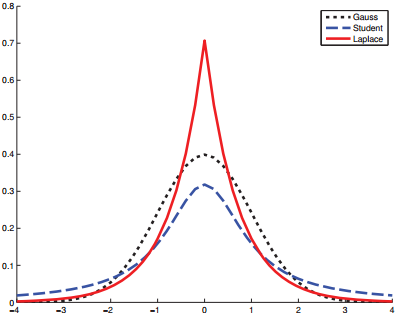
\includegraphics[scale=.70]{pdfs-for-NTL-a.png}} \\
\subfloat[]{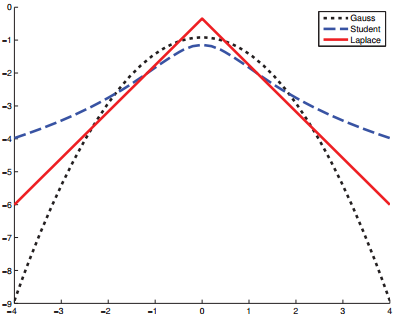
\includegraphics[scale=.70]{pdfs-for-NTL-b.png}}
\caption{(a)  $\mathcal{N}(0,1)$, $\mathcal{T}(0,1,1)$ এবং $Lap(0,1/\sqrt{2})$ {\bengalifont এর pdf, Gaussian এবং Laplace distribution এর জন্য mean 0 এবং variance 1। তবে যখন $\nu=1$, তখন Student distribution এর mean এবং variance undefined থাকে। }(b) {\bengalifont এই pdf গুলোর log; Student distribution কোন parameter মানেই log-concave নয়, অন্যদিকে Laplace distribution সবসময়ই log-concave (এবং log-convex...)। তা সত্ত্বেও, উভয়ই unimodal।
}}
%  %%%%%%%%%%%%%%%%%%%%%%%%%%%%%%%%%%%%%%% 
% should I add the defs of log concave, unimodal, log .....?
%  %%%%%%%%%%%%%%%%%%%%%%%%%%%%%%%%%%%%%%% 

\label{fig:pdfs-for-NTL} 
\end{figure}

{\bengalifont variance শুধুমাত্র $\nu>2$ হলে defined হয়। Mean শুধুমাত্র $\nu>1$ হলে defined হয়।}

{\bengalifont Student distribution এর robustness-এর ক্ষেত্রে, Figure \ref{fig:robustness}-এ আমরা দেখতে পাই যে Gaussian distribution অনেক বেশি প্রভাবিত হয়, কিন্তু Student distribution প্রায় অপরিবর্তিত থাকে। এর কারণ হল Student distribution এর তুলনামূলকভাবে ভারী tails (heavier tails) থাকে, বিশেষ করে যখন $\nu$ ছোট হয় (Figure \ref{fig:pdfs-for-NTL} দ্রষ্টব্য)।}

\begin{figure}[hbtp]
\centering
\subfloat[]{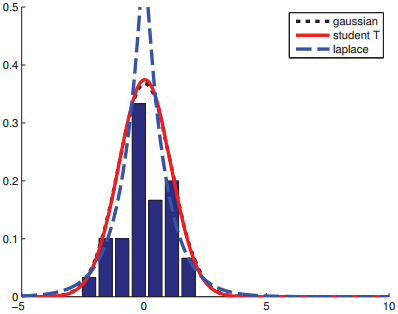
\includegraphics[scale=.70]{robustness-a.png}} \\
\subfloat[]{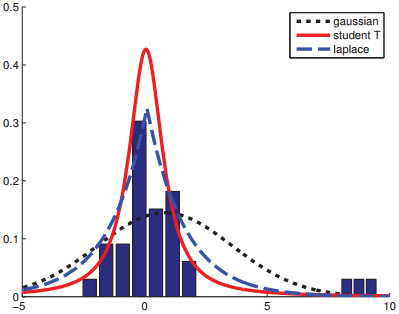
\includegraphics[scale=.70]{robustness-b.png}}
\caption{{\bengalifont Outliers এর প্রভাব Gaussian, Student এবং Laplace distribution ফিট করার উপর কেমন তা দেখানো হয়েছে। (a) যখন কোন outliers নেই (Gaussian এবং Student curves একটির উপর আরেকটি থাকে)। (b)  outliers সহ, Gaussian distribution outliers দ্বারা বেশি প্রভাবিত হয়, যেখানে Student এবং Laplace distributions তুলনামূলকভাবে কম প্রভাবিত হয়।}
}
\label{fig:robustness} 
\end{figure}
\bengalifont 
যদি $\nu=1$ হয়, তখন এই distribution কে \textbf{Cauchy} বা \textbf{Lorentz} distribution বলে। ভারী tails (heavy tails) থাকার জন্য পরিচিত, কারণ যেই integral দ্বারা mean সংজ্ঞায়িত করা হয় তা converge করে না।
 finite variance নিশ্চিত করার জন্য, আমাদের $\nu>2$ প্রয়োজন। সাধারণত $\nu=4$ ব্যবহার করা হয়, যা বিভিন্ন সমস্যার ক্ষেত্রে ভালো performance দেয় (Lange et al. 1989)। যখন $\nu \gg 5$, তখন Student distribution দ্রুত Gaussian distribution এর কাছাকাছি চলে আসে এবং এর robustness এর সুবিধা হারিয়ে ফেলে।


\subsection{The Laplace distribution}


\begin{table}
\caption{Summary of Laplace distribution.}
\centering
\begin{tabular}{cccccc}
\hline\noalign{\smallskip}
Written as & $f(x)$ & $\mathbb{E}[X]$ & mode & $\text{var}[X]$ \\
\noalign{\smallskip}\svhline\noalign{\smallskip}
$X \sim \text{Lap}(\mu,b)$ & $\dfrac{1}{2b}\exp\left(-\dfrac{|x-\mu|}{b}\right)$ & $\mu$ & $\mu$ & $2b^2$ \\
\noalign{\smallskip}\hline
\end{tabular}
\end{table}
{\bengalifont এখানে $\mu$ একটি location parameter এবং $b>0$ একটি scale parameter। Figure \ref{fig:pdfs-for-NTL} তে একটি plot}
{\bengalifont Laplace distribution এর robustness outliers Figure \ref{fig:robustness}-এ দেখানো হয়েছে। এটি Gaussian এর চেয়ে 0 এর দিকে বেশি probability density রাখে। এই বৈশিষ্ট্যটি একটি মডেলে sparsity (সম্প্রসারণ) বাড়াতে বেশ কার্যকর, যা আমরা Section TODO তে দেখতে পাবো।}



\subsection{The gamma distribution}

\begin{table}
\caption{Summary of gamma distribution}
\centering
\begin{tabular}{ccccccc}
\hline\noalign{\smallskip}
Written as & $X$ & $f(x)$ & $\mathbb{E}[X]$ & mode & $\text{var}[X]$ \\
\noalign{\smallskip}\svhline\noalign{\smallskip}
$X \sim \text{Ga}(a,b)$ & $x \in \mathbb{R}^+$ & $\dfrac{b^a}{\Gamma(a)}x^{a-1}e^{-xb}$ & $\dfrac{a}{b}$ & $\dfrac{a-1}{b}$ & $\dfrac{a}{b^2}$ \\
\noalign{\smallskip}\hline
\end{tabular}
\end{table} 
% {\bengalifont এখানে $a>0$ shape parameter এবং  $b>0$  rate parameter; \ref{fig:gamma-distribution} দ্রষ্টব্য}
Here  is called the  and. See Figure  for some plots.

\begin{figure}[hbtp]
\centering
\subfloat[]{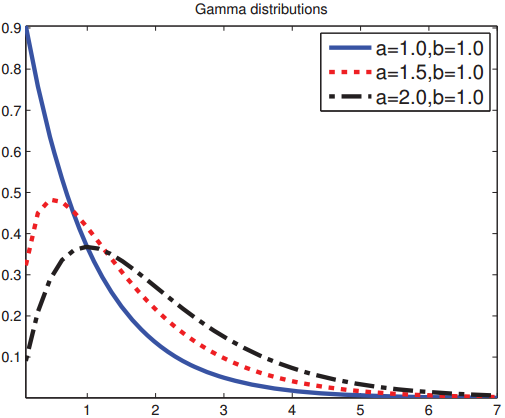
\includegraphics[scale=.50]{gamma-distribution-a.png}} \\
\subfloat[]{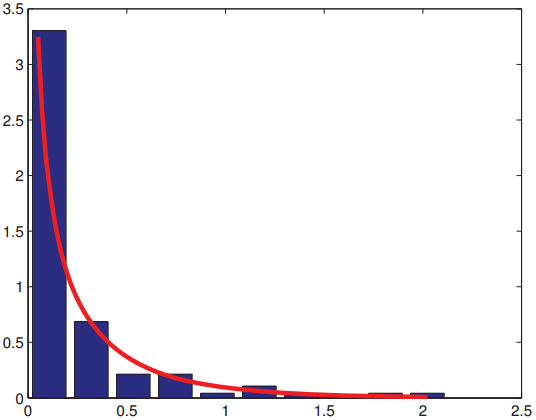
\includegraphics[scale=.50]{gamma-distribution-b.png}}
\caption{{\bengalifont কিছু Ga$(a, b=1)$ distributions। যদি $a \leq 1$ হয়, তাহলে mode 0-তে থাকে, অন্যথায় এটি $>0$ হয়। যখন আমরা $b$-এর rate বাড়াই, তখন আমরা horizontal scale কমাই, ফলে সবকিছু বাম দিকে এবং উপরের দিকে সঙ্কুচিত হয়। (b) কিছু বৃষ্টিপাতের ডেটার একটি empirical pdf, যেখানে একটি fitted Gamma distribution superimposed করা হয়েছে।}}

    % Some Ga$(a, b=1)$ distributions. If $a \leq 1$, the mode is at 0, otherwise it is $>0$.As we increase the rate $b$, we reduce the horizontal scale, thus squeezing everything leftwards and upwards. (b) An empirical pdf of some rainfall data, with a fitted Gamma distribution superimposed.}
\label{fig:gamma-distribution} 
\end{figure}


\subsection{The beta distribution}

\begin{table*}
\caption{Summary of Beta distribution}\label{tab:beta-distribution}
\centering
\begin{tabular}{ccccccc}
\hline\noalign{\smallskip}
Name & Written as & $X$ & $f(x)$ & $\mathbb{E}[X]$ & mode & $\text{var}[X]$ \\
\noalign{\smallskip}\svhline\noalign{\smallskip}
Beta distribution & $X \sim \text{Beta}(a,b)$ & $x \in [0,1]$ & $\dfrac{1}{B(a,b)}x^{a-1}(1-x)^{b-1}$ & $\dfrac{a}{a+b}$ & $\dfrac{a-1}{a+b-2}$ & $\dfrac{ab}{(a+b)^2(a+b+1)}$ \\
\noalign{\smallskip}\hline
\end{tabular}
\end{table*} 

Here $B(a, b)$is the beta function,
\begin{equation}
B(a,b) \triangleq \dfrac{\Gamma(a)\Gamma(b)}{\Gamma(a+b)}
\end{equation}
{\bengalifont কিছু beta distributions এর plot এর জন্য Figure \ref{fig:beta-distribution} দ্রষ্টব্য।  Distribution কে integrable করতে (অর্থাৎ $B(a, b)$ কে রাখার জন্যে), আমাদের $a, b >0$ প্রয়োজন। যদি $a=b=1$ হয়, আমরা uniform distribution পাই। যদি $a$ এবং $b$ উভয়ই 1 এর চেয়ে কম হয়, আমরা 0 এবং 1 এ "spikes" সহ একটি bimodal distribution পাই; যদি $a$ এবং $b$ উভয়ই 1 এর চেয়ে বড় হয়, distribution unimodal হয়।}


\begin{figure}[hbtp]
\centering
    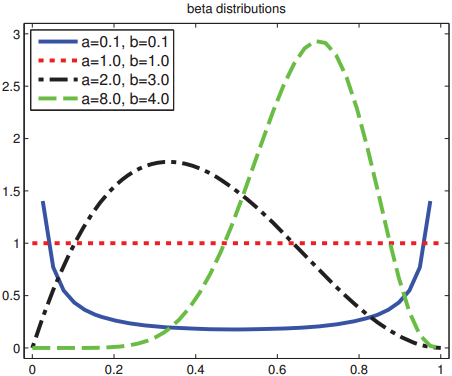
\includegraphics[scale=.60]{beta-distribution.png}
\caption{beta distribution}
\label{fig:beta-distribution} 
\end{figure}


\subsection{Pareto distribution}

\begin{table*}
\caption{Summary of Pareto distribution}
\centering
\begin{tabular}{ccccccc}
\hline\noalign{\smallskip}
Name & Written as & $X$ & $f(x)$ & $\mathbb{E}[X]$ & mode & $\text{var}[X]$ \\
\noalign{\smallskip}\svhline\noalign{\smallskip}
Pareto distribution & $X \sim \text{Pareto}(k,m)$ & $x \geq m$ & $km^kx^{-(k+1)}\mathbb{I}(x \geq m)$ & $\dfrac{km}{k-1} \text{ if } k > 1$ & $m$ & $\dfrac{m^2k}{(k-1)^2(k-2)} \text{ if } k>2$ \\
\noalign{\smallskip}\hline
\end{tabular}
\end{table*} 

The \textbf{Pareto distribution} is used to model the distribution of quantities that exhibit \textbf{long tails}, also called \textbf{heavy tails}.

As $k \rightarrow \infty$, the distribution approaches $\delta(x-m)$. See Figure \ref{fig:Pareto-distribution}(a) for some plots. If we plot the distribution on a log-log scale, it forms a straight line, of the form $\log p(x)=a\log x+c$ for some constants $a$ and $c$. See Figure \ref{fig:Pareto-distribution}(b) for an illustration (this is known as a \textbf{power law}).

\begin{figure}[hbtp]
\centering
\subfloat[]{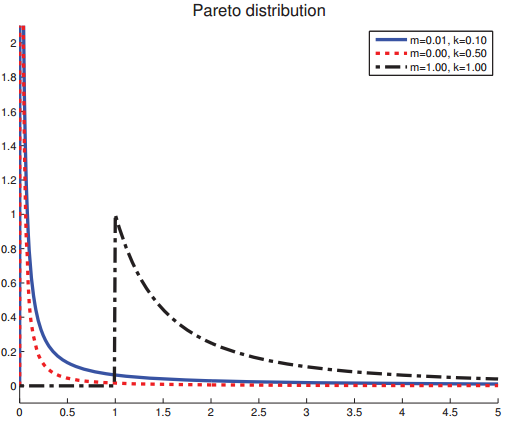
\includegraphics[scale=.50]{pareto-distribution-a.png}} \\
\subfloat[]{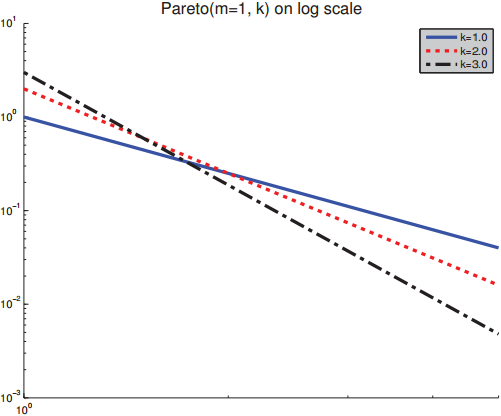
\includegraphics[scale=.50]{pareto-distribution-b.png}}
\caption{(a) The Pareto distribution Pareto$(x|m, k)$ for $m=1$. (b) The pdf on a log-log scale.}
\label{fig:Pareto-distribution} 
\end{figure}


\section{Joint probability distributions}
{\bengalifont ধরি একটি \textbf{multivariate random variable} বা \textbf{random vector} \footnote{\url{http://en.wikipedia.org/wiki/Multivariate_random_variable}} $X \in \mathbb{R}^D$, এর \textbf{joint probability distribution} \footnote{\url{http://en.wikipedia.org/wiki/Joint_probability_distribution}} হল একটি probability distribution যা নির্দেশ করে যে $X_1, X_2, \cdots,X_D$ এর প্রতিটি নির্দিষ্ট ভ্যালু বা নির্দিষ্ট রেঞ্জে পড়ার সম্ভাবনা কত। }

{\bengalifont যখন মাত্র দুটি random variable থাকে, তখন একে \textbf{bivariate distribution} বলা হয়, কিন্তু যেকোন সংখ্যক random variables এর ক্ষেত্রে generalized করা হলে তাকে  \textbf{multivariate distribution} বলে।}

{\bengalifont Joint probability distribution কে প্রকাশ করা যেতে পারে \textbf{joint cumulative distribution function} এর মাধ্যমে, অথবা \textbf{joint probability density function} এর মাধ্যমে (যদি variables continuous হয়) অথবা \textbf{joint probability mass function} এর মাধ্যমে (যদি variables discrete হয়)।}




\subsection{Covariance and correlation}
\begin{definition}

{\bengalifont Covariance} হল দুইটি random variables $X$ এবং $Y$ এর মধ্যে কতটুকু (বা কত ডিগ্রী পর্যন্ত) linearity আছে তা পরিমাপ করে। Covariance কে নিম্নরূপে সংজ্ঞায়িত করা হয়েছে:

\begin{equation}
\begin{split}
\mathrm{cov}[X,Y] & \triangleq \mathbb{E}\left[(X-\mathbb{E}[X])(Y-\mathbb{E}[Y])\right] \\
         & =\mathbb{E}[XY]-\mathbb{E}[X]\mathbb{E}[Y]
\end{split}
\end{equation}
\end{definition}

\begin{definition}
{\bengalifont যদি $X$ একটি $D$-dimensional random vector হয়, তাহলে এর {\textbf covariance matrix} কে নিম্নরূপ symmetric, positive definite matrix হিসেবে সংজ্ঞায়িত করা হয়:}

If $X$ is a $D$-dimensional random vector, its \textbf{covariance matrix} is defined to be the following symmetric, positive definite matrix:
\begin{align}
\mathrm{cov}[X] & \triangleq \mathbb{E}\left[(X-\mathbb{E}[X])(X-\mathbb{E}[X])^T\right] \\
       &  = \left( \begin{array}{cccc}
           \text{var}[X_1] & \text{Cov}[X_1,X_2] & \cdots & \text{Cov}[X_1,X_D] \\
           \text{Cov}[X_2,X_1] & \text{var}[X_2] & \cdots & \text{Cov}[X_2,X_D] \\
		   \vdots & \vdots & \ddots & \vdots \\
           \text{Cov}[X_D,X_1] & \text{Cov}[X_D,X_2] & \cdots & \text{var}[X_D] \end{array} \right)
\end{align}
\end{definition}

\begin{definition}
{\bengalifont  $X$ এবং $Y$ এর মধ্যে(Pearson) {\textbf correlation coefficient} :}

\begin{equation}
\text{corr}[X,Y] \triangleq \dfrac{\text{Cov}[X,Y]}{\sqrt{\text{var}[X],\text{var}[Y]}}
\end{equation}
\end{definition}

A \textbf{correlation matrix} has the form
\begin{equation}
\mathbf{R} \triangleq \left( \begin{array}{cccc}
           \text{corr}[X_1,X_1] & \text{corr}[X_1,X_2] & \cdots & \text{corr}[X_1,X_D] \\
           \text{corr}[X_2,X_1] & \text{corr}[X_2,X_2] & \cdots & \text{corr}[X_2,X_D] \\
		   \vdots & \vdots & \ddots & \vdots \\
           \text{corr}[X_D,X_1] & \text{corr}[X_D,X_2] & \cdots & \text{corr}[X_D,X_D] \end{array} \right)
\end{equation}

\begin{figure*}[hbtp]
\centering
    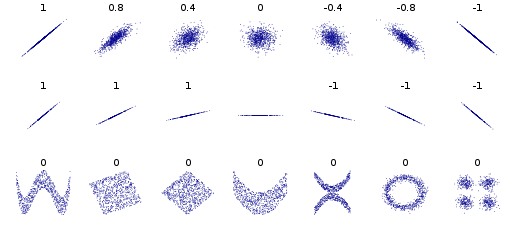
\includegraphics[scale=.80]{Correlation-examples.png}
\caption{ {\bengalifont বেশ কিছু $(x, y)$ points এর সেটে, $x$ এবং $y$ এর মধ্যে Pearson correlation coefficient নির্ধারণ করা হয়েছে। লক্ষ্য করি যে, correlation একটা linear  relation direction এবং noisiness নির্দেশ করে, তবে সেই সম্পর্কের slope নির্দেশ করে না (মাঝের সারি), এবং নন-লিনিয়ার সম্পর্কের অনেক দিকও নির্দেশ করে না (নিচের সারি)। নোটঃ মাঝখানের ছবিটির slope 0, কিন্তু এই ক্ষেত্রে correlation coefficient নির্ধারিত হয়নি কারণ $Y$ এর variance শূন্য। রেফারেন্স :\url{http://en.wikipedia.org/wiki/Correlation}}}

\label{fig:Correlation-examples} 
\end{figure*}

\textbf{Uncorrelated does not imply independent}. {\bengalifont উদাহরণস্বরূপ, যদি $X \sim U(-1,1)$ এবং $Y = X^2$, $Y$ যদি $X$ এর উপর নির্ভরশীল,  একে দেখানো যায় যে $ \text{corr}[X, Y]=0$। Figure \ref{fig:Correlation-examples} এ এই বিষয়টি কিছু উদাহরণ সহ দেখানো হয়েছে যেখানে $X$ এবং $Y$ এর মধ্যে স্পষ্ট সম্পর্ক রয়েছে, কিন্তু correlation coefficient 0। Random variables এর মধ্যে আরও সাধারণ একটি dependence-এর পরিমাপ হল \textbf{mutual information}; বিস্তারিত Section TODO তে।}



\subsection{Multivariate Gaussian distribution}
\label{sec:MVN}
The \textbf{multivariate Gaussian} or \textbf{multivariate normal}(MVN) is the most widely used joint probability density function for continuous variables. We discuss MVNs in detail in Chapter 4; here we just give some definitions and plots.

The pdf of the MVN in $D$ dimensions is defined by the following:
\begin{equation}
\mathcal{N}(\vec{x}|\vec{\mu},\Sigma) \triangleq \dfrac{1}{(2\pi)^{D/2}|\Sigma|^{1/2}}\exp\left[-\dfrac{1}{2}(\vec{x}-\vec{\mu})^T\Sigma^{-1}(\vec{x}-\vec{\mu})\right]
\end{equation}
where $\vec{\mu}=\mathbb{E}[X] \in \mathbb{R}^D$ is the mean vector, and $\Sigma=\text{Cov}[X]$ is the $D \times D$ covariance matrix. The normalization constant $(2\pi)^{D/2}|\Sigma|^{1/2}$ just ensures that the pdf integrates to 1.

Figure \ref{fig:2d-Gaussions} plots some MVN densities in 2d for three different kinds of covariance matrices. A full covariance matrix has A $D(D+1)/2$ parameters (we divide by 2 since $\Sigma$ is symmetric). A diagonal covariance matrix has $D$ parameters, and has 0s in the off-diagonal terms. A spherical or isotropic covariance,$\Sigma=\sigma^2\vec{I}_D$, has one free parameter.

\begin{figure}[hbtp]
\centering
\subfloat[]{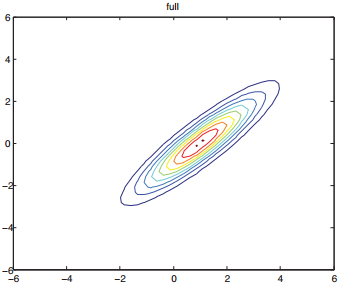
\includegraphics[scale=.60]{2d-Gaussions-a.png}} \\
\subfloat[]{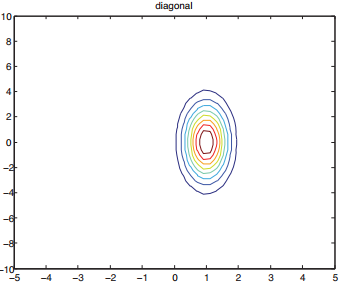
\includegraphics[scale=.60]{2d-Gaussions-b.png}} \\
\subfloat[]{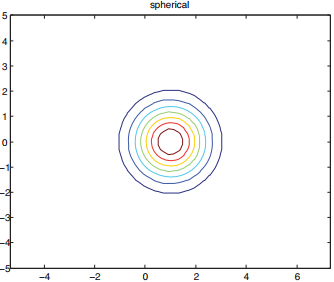
\includegraphics[scale=.60]{2d-Gaussions-c.png}} \\
\subfloat[]{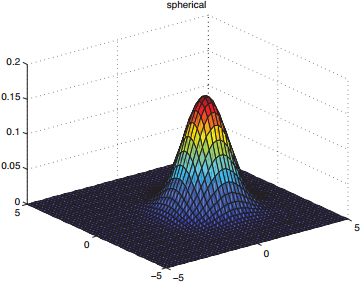
\includegraphics[scale=.60]{2d-Gaussions-d.png}}
\caption{We show the level sets for 2d Gaussians. (a) A full covariance matrix has elliptical contours.(b) A diagonal covariance matrix is an axis aligned ellipse. (c) A spherical covariance matrix has a circular shape. (d) Surface plot for the spherical Gaussian in (c).}
\label{fig:2d-Gaussions} 
\end{figure}


\subsection{Multivariate Student's t-distribution}
A more robust alternative to the MVN is the multivariate Student's t-distribution, whose pdf is given by
\begin{align}
& \mathcal{T}(x|\vec{\mu},\Sigma,\nu) \nonumber \\
& \triangleq \dfrac{\Gamma(\frac{\nu+D}{2})}{\Gamma(\frac{\nu}{2})}\dfrac{|\Sigma|^{-\frac{1}{2}}}{\left(\nu\pi\right)^{\frac{D}{2}}}\left[1+\dfrac{1}{\nu}\left(\vec{x}-\vec{\mu}\right)^T\Sigma^{-1}\left(\vec{x}-\vec{\mu}\right)\right]^{-\frac{\nu+D}{2}} \\
&= \dfrac{\Gamma(\frac{\nu+D}{2})}{\Gamma(\frac{\nu}{2})}\dfrac{|\Sigma|^{-\frac{1}{2}}}{\left(\nu\pi\right)^{\frac{D}{2}}}\left[1+\left(\vec{x}-\vec{\mu}\right)^T\vec{V}^{-1}\left(\vec{x}-\vec{\mu}\right)\right]^{-\frac{\nu+D}{2}}
\end{align}
where $\Sigma$ is called the scale matrix (since it is not exactly the covariance matrix) and $\vec{V}=\nu\Sigma$. This has fatter tails than a Gaussian. The smaller $\nu$ is, the fatter the tails. As $\nu \rightarrow \infty$, the distribution tends towards a Gaussian. The distribution has the following properties
\begin{equation}
\text{mean}=\vec{\mu} \text{ , mode}=\vec{\mu} \text{ , Cov}= \dfrac{\nu}{\nu-2}\Sigma
\end{equation}


\subsection{Dirichlet distribution}
A multivariate generalization of the beta distribution is the \textbf{Dirichlet distribution}, which has
support over the probability simplex, defined by
\begin{equation}
S_K=\left\{\vec{x}:0 \leq x_k \leq 1,\sum\limits_{k=1}^K x_k=1\right\}
\end{equation}

The pdf is defined as follows:
\begin{equation}
\text{Dir}(\vec{x}|\vec{\alpha}) \triangleq \dfrac{1}{B(\vec{\alpha})}\prod\limits_{k=1}^K x_k^{\alpha_k-1}\mathbb{I}(\vec{x} \in S_K)
\end{equation}
where $B(\alpha_1,\alpha_2,\cdots,\alpha_K)$ is the natural generalization of the beta function to $K$ variables:
\begin{equation}
B(\alpha) \triangleq \dfrac{\prod_{k=1}^K \Gamma(\alpha_k)}{\Gamma(\alpha_0)} \text{ where } \alpha_0 \triangleq \sum_{k=1}^K \alpha_k
\end{equation}

Figure \ref{fig:3d-Dirichlet} shows some plots of the Dirichlet when $K=3$, and Figure \ref{fig:5d-Dirichlet} for some sampled probability vectors. We see that $\alpha_0$ controls the strength of the distribution (how peaked it is), and theαkcontrol where the peak occurs. For example, Dir$(1,1,1)$ is a uniform distribution, Dir$(2,2,2)$ is a broad distribution centered at $(1/3,1/3,1/3)$, and Dir$(20,20,20)$ is a narrow distribution centered at $(1/3,1/3,1/3)$.If $\alpha_k < 1$ for all $k$, we get “spikes” at the corner of the simplex.

\begin{figure}[hbtp]
\centering
\subfloat[]{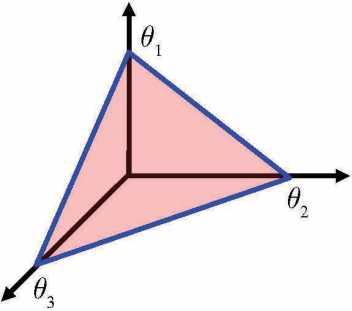
\includegraphics[scale=.50]{3d-Dirichlet-a.png}} \\
\subfloat[]{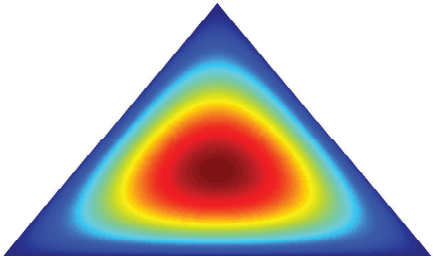
\includegraphics[scale=.60]{3d-Dirichlet-b.png}} \\
\subfloat[]{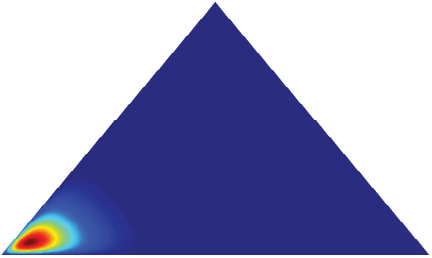
\includegraphics[scale=.60]{3d-Dirichlet-c.png}} \\
\subfloat[]{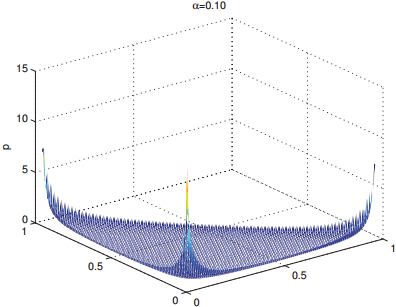
\includegraphics[scale=.60]{3d-Dirichlet-d.png}}
\caption{(a) The Dirichlet distribution when $K=3$ defines a distribution over the simplex, which can be represented by the triangular surface. Points on this surface satisfy $0 \leq \theta_k \leq 1$ and $\sum_{k=1}^K \theta_k=1$. (b) Plot of the Dirichlet density when $\vec{\alpha}=(2,2,2)$. (c) $\vec{\alpha}=(20,2,2)$.}
\label{fig:3d-Dirichlet} 
\end{figure}

\begin{figure}[hbtp]
\centering
\subfloat[$\vec{\alpha}=(0.1,\cdots,0.1)$. This results in very sparse distributions, with many 0s.]{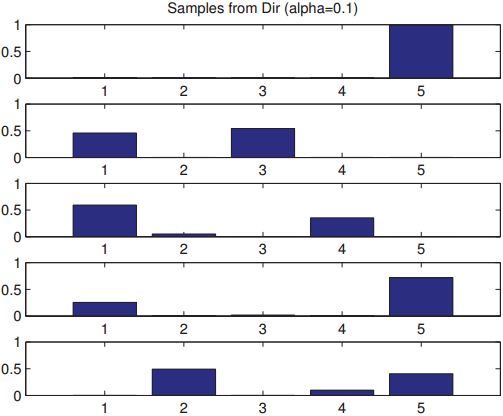
\includegraphics[scale=.50]{5d-Dirichlet-a.png}} \\
\subfloat[$\vec{\alpha}=(1,\cdots,1)$. This results in more uniform (and dense) distributions.]{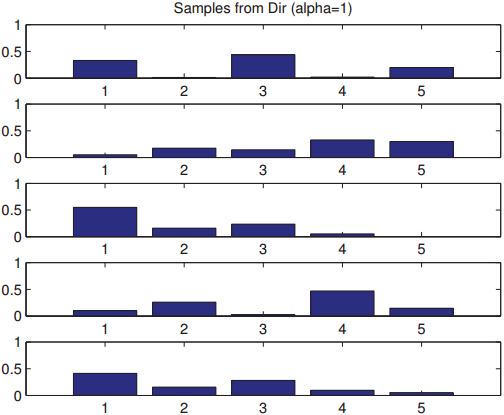
\includegraphics[scale=.50]{5d-Dirichlet-b.png}}
\caption{Samples from a 5-dimensional symmetric Dirichlet distribution for different parameter values.} 
\label{fig:5d-Dirichlet} 
\end{figure}

For future reference, the distribution has these properties
\begin{equation}\label{eqn:Dirichlet-properties}
\mathbb{E}(x_k)=\dfrac{\alpha_k}{\alpha_0} \text{, mode}[x_k]=\dfrac{\alpha_k-1}{\alpha_0-K} \text{, var}[x_k]=\dfrac{\alpha_k(\alpha_0-\alpha_k)}{\alpha_0^2(\alpha_0+1)}
\end{equation}


\section{Transformations of random variables}
If $\vec{x} \sim P()$ is some random variable, and $\vec{y}=f(\vec{x})$, what is the distribution of $Y$? This is the question we address in this section.


\subsection{Linear transformations}
Suppose $g()$ is a linear function: 
\begin{equation}
g(\vec{x})=A\vec{x}+b
\end{equation}

First, for the mean, we have
\begin{equation}
\mathbb{E}[\vec{y}]=\mathbb{E}[A\vec{x}+b]=A\mathbb{E}[\vec{x}]+b
\end{equation}
this is called the \textbf{linearity of expectation}.

For the covariance, we have
\begin{equation}
\text{Cov}[\vec{y}]=\text{Cov}[A\vec{x}+b]=A\Sigma A^T
\end{equation}


\subsection{General transformations}
\label{sec:General-transformations}
If $X$ is a discrete rv, we can derive the pmf for $y$ by simply summing up the probability mass for all the $x$’s such that $f(x)=y$:
\begin{equation}\label{eqn:transformation-discrete}
p_Y(y)=\sum\limits_{x:g(x)=y}p_X(x)
\end{equation}

If $X$ is continuous, we cannot use Equation \ref{eqn:transformation-discrete} since $p_X(x)$ is a density, not a pmf, and we cannot sum up densities. Instead, we work with cdf’s, and write
\begin{equation}
F_Y(y)=P(Y \leq y)=P(g(X) \leq y)=\int\limits_{g(X) \leq y} f_X(x)\mathrm{d}x
\end{equation}

We can derive the pdf of $Y$ by differentiating the cdf:
\begin{equation}\label{eqn:General-transformations}
f_Y(y)=f_X(x)|\dfrac{dx}{dy}|
\end{equation}

This is called \textbf{change of variables} formula. We leave the proof of this as an exercise. 

For example, suppose $X \sim U(−1,1)$, and $Y=X^2$. Then $p_Y(y)=\dfrac{1}{2}y^{-\frac{1}{2}}$.


\subsubsection{Multivariate change of variables *}
Let $f$ be a function $f:\mathbb{R}^n \rightarrow \mathbb{R}^n$, and let $\vec{y}=f(\vec{x})$. Then its Jacobian matrix $\vec{J}$ is given by
\begin{equation}
\vec{J}_{\vec{x} \rightarrow \vec{y}} \triangleq \frac{\partial \vec{y}}{\partial \vec{x}} \triangleq \left(\begin{array}{ccc}
\frac{\partial y_1}{\partial x_1} & \cdots & \frac{\partial y_1}{\partial x_n} \\
\vdots & \vdots & \vdots \\
\frac{\partial y_n}{\partial x_1} & \cdots & \frac{\partial y_n}{\partial x_n}
\end{array}\right)
\end{equation}
$|\mathrm{det}(\vec{J})|$ measures how much a unit cube changes in volume when we apply $f$.

If $f$ is an invertible mapping, we can define the pdf of the transformed variables using the Jacobian of the inverse mapping $\vec{y} \rightarrow \vec{x}$:
\begin{equation}\label{eqn:Multivariate-transformation}
p_y(\vec{y})=p_x(\vec{x})|\mathrm{det}(\frac{\partial \vec{x}}{\partial \vec{y}})|=p_x(\vec{x})|\mathrm{det}(\vec{J}_{\vec{y} \rightarrow \vec{x}})|
\end{equation}


\subsection{Central limit theorem}
Given $N$ random variables $X_1,X_2,\cdots,X_N$, each variable is \textbf{independent and identically distributed}\footnote{\url{http://en.wikipedia.org/wiki/Independent_identically_distributed}}(\textbf{iid} for short), and each has the same mean $\mu$ and variance $\sigma^2$, then
\begin{equation}
\dfrac{\sum\limits_{i=1}^n X_i-N\mu}{\sqrt{N}\sigma} \sim \mathcal{N}(0,1)
\end{equation}
this can also be written as
\begin{equation}
\dfrac{\bar{X}-\mu}{\sigma/\sqrt{N}} \sim \mathcal{N}(0,1) \quad \text{, where } \bar{X} \triangleq \dfrac{1}{N}\sum\limits_{i=1}^n X_i
\end{equation}


\section{Monte Carlo approximation}
\label{sec:Monte-Carlo-approximation}
In general, computing the distribution of a function of an rv using the change of variables formula can be difficult. One simple but powerful alternative is as follows. First we generate $S$ samples from the distribution, call them $x_1,\cdots,x_S$. (There are many ways to generate such samples; one popular method, for high dimensional distributions, is called Markov chain Monte Carlo or MCMC; this will be explained in Chapter TODO.) Given the samples, we can approximate the distribution of $f(X)$ by using the empirical distribution of $\left\{f(x_s)\right\}_{s=1}^S$. This is called a \textbf{Monte Carlo approximation}\footnote{\url{http://en.wikipedia.org/wiki/Monte_Carlo_method}}, named after a city in Europe known for its plush gambling casinos.

We can use Monte Carlo to approximate the expected value of any function of a random variable. We simply draw samples, and then compute the arithmetic mean of the function applied to the samples. This can be written as follows:
\begin{equation}
\mathbb{E}[g(X)]=\int g(x)p(x)\mathrm{d}x \approx \dfrac{1}{S}\sum\limits_{s=1}^S f(x_s)
\end{equation}
where $x_s \sim p(X)$.

This is called \textbf{Monte Carlo integration}\footnote{\url{http://en.wikipedia.org/wiki/Monte_Carlo_integration}}, and has the advantage over numerical integration (which is based on evaluating the function at a fixed grid of points) that the function is only evaluated in places where there is non-negligible probability.


\section{Information theory}

\subsection{Entropy}
\label{sec:Entropy}
{\bengalifont একটি random variable $X$ এর entropy, যার distribution $p$ দ্বারা নির্ধারিত, এবং যেটা $\mathbb{H}(X)$ বা কখনও কখনও $\mathbb{H}(p)$ দ্বারা চিহ্নিত হয়, এটি random variable- এর  uncertainty এর একটি পরিমাপ। বিশেষ করে, যদি $X$ একটি discrete ভেরিয়েবল হয় যার $K$-টি states আছে, তবে এটি নিম্নরূপ সংজ্ঞায়িত করা হয়:}

% The entropy of a random variable $X$ with distribution $p$, denoted by $\mathbb{H}(X)$ or sometimes $\mathbb{H}(p)$, is a measure of its uncertainty. In particular, for a discrete variable with $K$ states, it is defined by
\begin{equation}
\mathbb{H}(X) \triangleq -\sum\limits_{k=1}^{K}{p(X=k)\log_2p(X=k)}
\end{equation}

\bengalifont
-    ইকুয়েশনটি একটি discrete random variable $X$ এর জন্য entropy, যেখানে $X$ এর একটি probability distribution $p$ রয়েছে

-   $\mathbb{H}(X)$: {\bengalifont এটি random variable $X$ এর entropy। Entropy দ্বারা $X$ এর distribution এ কতটা uncertainty বা randomness আছে সেটা হিসাব করা হচ্ছে }

-   $\sum\limits_{k=1}^{K}$: {\bengalifont এই summation চিহ্নটি নির্দেশ করে যে আমরা $X$ এর সমস্ত সম্ভাব্য states বা values এর উপর যোগফল নিচ্ছি, যেখানে $K$ হল states এর সংখ্যা।}

-   $p(X=k)$: {\bengalifont random variable $X$, $k$ এর একটি নির্দিষ্ট মান গ্রহণ করার সম্ভাবনা।  সুতরাং, $p(X=k)$ প্রতিটি state $k$ এর জন্য probability নির্দেশ করে।}

- $\log_2 p(X=k)$: {\bengalifont এটি $p(X=k)$ এর base 2 logarithm। এখানে base 2 logarithm ব্যবহার করা হচ্ছে কারণ entropy কে "bits" এ পরিমাপ করা হচ্ছে, যা digital systems এর ক্ষেত্রে প্রযোজ্য।}

- {\bengalifont entropy-এর সম্পূর্ণ সমীকরণ}: {\bengalifont এই সমীকরণটি প্রতিটি probability $p(X=k)$ কে তার লগারিদম $\log_2 p(X=k)$ এর সাথে গুণ করে, তারপর সমস্ত states $k$ এর জন্য যোগ করে, এবং শেষে এটিকে -1 দ্বারা গুণ করা হচ্ছে।}

{\bengalifont 
### এর কাজ কী:
Entropy পরিমাপ করে একটি probability distribution এর মধ্যে কতটা uncertainty বা information content রয়েছে। সহজ ভাষায়, এটি আমাদের বলে দেয় কতটা unpredictable হবে random variable $X$ এর মান।}

- {\bengalifont যদি সমস্ত states সমান সম্ভাবনা নিয়ে থাকে, তাহলে entropy বেশি হবে, কারণ $X$ এর মান সহজে পূর্বানুমান করা যায় না।}

- {\bengalifont যদি একটি state এর সমস্ত সম্ভাবনা থাকে (i.e., certaintly), তবে entropy কম বা শূন্য হবে, কারণ এখানে কোনও uncertainty নেই।}


{\bengalifont সাধারণত আমরা log এর base 2 ব্যবহার করি, এবং এই ক্ষেত্রে এর units কে \textbf{bits} (binary digits এর সংক্ষিপ্ত রূপ) বলা হয়। যদি আমরা log এর base $e$ ব্যবহার করি, units গুলোকে \textbf{nats} বলা হয়।}

{\bengalifont সর্বোচ্চ entropy সহ একটি discrete distribution হল uniform distribution (প্রমাণের জন্য Section XXX দ্রষ্টব্য)। সুতরাং, যদি একটি $K$-ary random variable এর ক্ষেত্রে $p(x=k) = 1/K$, তাহলে entropy সর্বাধিক হয়; এই ক্ষেত্রে $\mathbb{H}(X) = \log_2 K$।}

{\bengalifont বিপরীতভাবে, সর্বনিম্ন entropy সহ একটি distribution (যা শূন্য) হল যেকোনো \textbf{delta-function}, যা এর সব mass একটি state এ ধরে রাখে। এমন একটি distribution এ কোনো uncertainty থাকে না।}


\subsection{KL divergence}
One way to measure the dissimilarity of two probability distributions, $p$ and $q$ , is known as the \textbf{Kullback-Leibler divergence}(\textbf{KL divergence})or \textbf{relative entropy}. This is defined as follows:
\begin{equation}
\mathbb{KL}(P||Q) \triangleq 
\sum\limits_{x}{p(x)\log_2\dfrac{p(x)}{q(x)}}
\end{equation}
where the sum gets replaced by an integral for pdfs\footnote{The KL divergence is not a distance, since it is asymmetric. One symmetric version of the KL divergence is the \textbf{Jensen-Shannon divergence}, defined as $JS(p_1,p_2)=0.5\mathbb{KL}(p_1||q)+0.5\mathbb{KL}(p_2||q)$,where $q=0.5p_1+0.5p_2$}. The KL divergence is only defined if P and Q both sum to 1 and if $q(x)=0$ implies $p(x)=0$ for all $x$(absolute continuity). If the quantity  $0\ln0$ appears in the formula, it is interpreted as zero because $\lim\limits_{x \to 0}x\ln x$. We can rewrite this as
\begin{equation}\begin{split}
\mathbb{KL}(p||q) & \triangleq \sum\limits_{x}{p(x)\log_2p(x)}-\sum\limits_{k=1}^{K}{p(x)\log_2q(x)} \\
    & =\mathbb{H}(p,q)-\mathbb{H}(p)
\end{split}\end{equation}
where $\mathbb{H}(p,q)$ is called the \textbf{cross entropy},
\begin{equation}\label{eqn:cross-entropy}
\mathbb{H}(p,q)=-\sum\limits_{x}{p(x)\log_2q(x)}
\end{equation}

One can show (Cover and Thomas 2006) that the cross entropy is the average number of bits needed to encode data coming from a source with distribution $p$ when we use model $q$ to define our codebook. Hence the “regular” entropy $\mathbb{H}(p)=\mathbb{H}(p,p)$, defined in section \S \ref{sec:Entropy},is the expected number of bits if we use the true model, so the KL divergence is the diference between these. In other words, the KL divergence is the average number of \emph{extra} bits needed to encode the data, due to the fact that we used distribution $q$ to encode the data instead of the true distribution $p$.

The “extra number of bits” interpretation should make it clear that $\mathbb{KL}(p||q) \geq 0$, and that the KL is only equal to zero if $q = p$. We now give a proof of this important result.

\begin{theorem}
(\textbf{Information inequality}) $\mathbb{KL}(p||q) \geq 0 \text{ with equality iff } p=q$.
\end{theorem}

One important consequence of this result is that \emph{the discrete distribution with the maximum
entropy is the uniform distribution}.


\subsection{Mutual information}
\label{sec:Mutual-information}
\begin{definition}
\textbf{Mutual information} or \textbf{MI}, is defined as follows:
\begin{equation}\begin{split}
\mathbb{I}(X;Y) & \triangleq \mathbb{KL}(P(X,Y)||P(X)P(Y)) \\
    & =\sum\limits_x\sum\limits_yp(x,y)\log\dfrac{p(x,y)}{p(x)p(y)}
\end{split}\end{equation}
We have $\mathbb{I}(X;Y) \geq 0$ with equality if $P(X,Y)=P(X)P(Y)$. That is, the MI is zero if the variables are independent.
\end{definition}

To gain insight into the meaning of MI, it helps to re-express it in terms of joint and conditional entropies. One can show that the above expression is equivalent to the following:
\begin{eqnarray}
\mathbb{I}(X;Y)&=&\mathbb{H}(X)-\mathbb{H}(X|Y)\\
               &=&\mathbb{H}(Y)-\mathbb{H}(Y|X)\\
               &=&\mathbb{H}(X)+\mathbb{H}(Y)-\mathbb{H}(X,Y)\\
               &=&\mathbb{H}(X,Y)-\mathbb{H}(X|Y)-\mathbb{H}(Y|X)
\end{eqnarray}
where $\mathbb{H}(X)$ and $\mathbb{H}(Y)$ are the \textbf{marginal entropies}, $\mathbb{H}(X|Y)$ and $\mathbb{H}(Y|X)$ are the \textbf{conditional entropies}, and $\mathbb{H}(X,Y)$ is the \textbf{joint entropy} of $X$ and $Y$, see Fig. \ref{fig:mi}\footnote{\url{http://en.wikipedia.org/wiki/Mutual_information}}.

\begin{figure}[hbtp]
\centering
    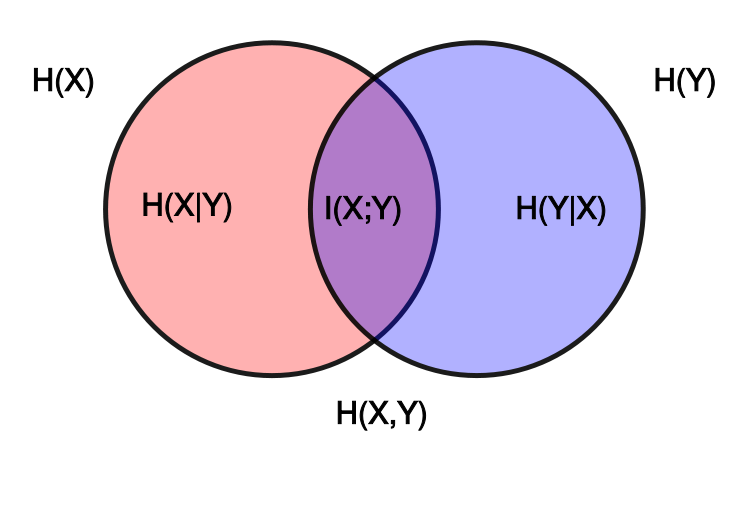
\includegraphics[scale=.25]{mutual-information.png}
\caption{Individual $\mathbb{H}(X),\mathbb{H}(Y)$, joint $\mathbb{H}(X,Y)$, and conditional entropies for a pair of correlated subsystems $X,Y$ with mutual information $\mathbb{I}(X;Y)$.}
\label{fig:mi} 
\end{figure}

Intuitively, we can interpret the MI between $X$ and $Y$ as the reduction in uncertainty about $X$ after observing $Y$, or, by symmetry, the reduction in uncertainty about $Y$ after observing $X$.

A quantity which is closely related to MI is the \textbf{pointwise mutual information} or \textbf{PMI}. For two events (not random variables) $x$ and $y$, this is defined as
\begin{equation}
PMI(x,y) \triangleq \log\dfrac{p(x,y)}{p(x)p(y)}=\log\dfrac{p(x|y)}{p(x)}=\log\dfrac{p(y|x)}{p(y)}
\end{equation}

This measures the discrepancy between these events occuring together compared to what would be expected by chance. Clearly the MI of $X$ and $Y$ is just the expected value of the PMI. Interestingly, we can rewrite the PMI as follows:
\begin{equation}
PMI(x,y)=\log\dfrac{p(x|y)}{p(x)}=\log\dfrac{p(y|x)}{p(y)}
\end{equation}

This is the amount we learn from updating the prior $p(x)$ into the posterior $p(x|y)$, or equivalently, updating the prior $p(y)$ into the posterior $p(y |x)$.


\end{document}